\documentclass[twocolumn]{article} % Or your preferred document class and options
% !TEX root = main.tex

\usepackage{preamble} % Load your custom preamble


\begin{document}

\coverpage

\begin{abstract}
    abc
\end{abstract}


\section{Introduction}

Quantum-inspired algorithms are classical routines that use mathematical structures and physical intuitions from quantum mechanics — such as superposition-style probability amplitudes, interference or quantum state discrimination — yet run entirely on conventional hardware.  
These algorithms have multiple applications, including machine learning, where they promise faster convergence or reduced dimensional dependence compared with traditional methods.

Some machine-learning algorithms are based on distance. 
Here, the decision rule depends on the similarity between a query sample and a set of prototypes, typically evaluated through dot products or euclidean distance calculation.  Although straightforward in software, these operations become a computational bottleneck for high-dimensional data streams or large datasets.  
There have been optical implementations of classical classification algorithms (\cite{Neifeld1993}, \cite{Foor1995}). These implementations offer a compelling alternative: coherent light can perform calculations at the speed of propagation, exploiting spatial parallelism while consuming only milliwatts of power.

Among the various optical architectures, the \emph{Joint Transform Correlator} (JTC) (\cite{Psaltis1984}, \cite{Dragulinescu2023}) stands out for its simplicity and adaptability.  Unlike classical VanderLugt systems (\cite{VanderLugt1964}), the JTC does not require a pre-fabricated filter; instead, the reference and query patterns are placed side by side in the input plane.  A single Fourier transform—implemented with a lens—produces an output intensity whose off-axis terms encode the cross-correlation between the two patterns.  
When feature vectors are encoded as two-dimensional phase distributions, the correlation peak height provides a direct measure of their similarity, which can be mapped to a distance-based decision rule.

In this work we propose optical implementations of the Quantum-Inspired and Classical Nearest Mean Classifier (\cite{Cruzeiro2024}, \cite{Sergioli2025}), and Radial Basis Function Classifier (\cite{Neifeld1993}, \cite{Foor1995}), that use a single SLM and a 1-f lens system (\cite{Javidi1989}).  We begin by reviewing the theoretical connection between optical correlation and amplitude-based similarity measures. We then describe our experimental set-up, which integrates a single reflective, phase only, spatial light modulator and a CMOS camera to implement a proof-of-concept optical classifier (Section~\ref{sec:setup}).  Finally, we benchmark the models with the MNIST dataset and compare their performances with purely electronic implementations, highlighting the trade-offs in speed, energy, and classification accuracy (Section~\ref{sec:results}).


\section{Theory}

\subsection{Machine learning and supervised learning}

\label{subsec:ml}

Machine learning (ML) provides algorithmic tools that \emph{learn}
directly from data rather than relying on hand-crafted rules.
In the \emph{supervised} setting, learning is guided by \emph{examples}
whose correct answers are known in advance.  We review the key
ingredients used throughout this work.

\paragraph{Input data.}
We start from $N$ \emph{raw samples}
\(
\mathbf u_i\in\mathbb R^{p},\; i=1,\dots,N,
\)
each accompanied by a \emph{label}
\(
y_i\in\{1,\dots,K\}.
\)
The labels partition the data into
\[
C_k=\{\mathbf u_i: y_i=k\},
\qquad
N_k=|C_k|,
\qquad
p_k=\frac{N_k}{N},
\]
where $N_k$ and $p_k$ are the size and empirical probability of class
$k$, respectively.  It is convenient to organise the entire data set as
a matrix
$
\mathbf M=[\mathbf u_1\;\mathbf u_2\;\cdots\;\mathbf u_N]\in\mathbb R^{p\times N}
$
and the labels as a vector
$
\mathbf y=[y_1,\dots,y_N]^{\!\top}\!.
$

\paragraph{Training and test sets.}
A \emph{training set}
$(\mathbf M_{\text{train}},\mathbf y_{\text{train}})$
is used to tune the parameters of a classifier, while a disjoint
\emph{test set}
$(\mathbf M_{\text{test}},\mathbf y_{\text{test}})$
gauges its ability to generalise to unseen data. 
The algorithm is trained on the training set and evaluated on the test set. In this work we will be using the MNIST dataset (Fig.\ref{fig:mnist-examples}), with $60000$ training samples and $10000$ testing samples.

\begin{figure}[htbp]
  \centering
  % Replace digits_0.png ... digits_9.png with your own 28x28 PNGs
  \setlength{\tabcolsep}{2pt}
  \renewcommand{\arraystretch}{0}
  \begin{tabular}{ccccc} % Changed from 10 c's to 5 c's
    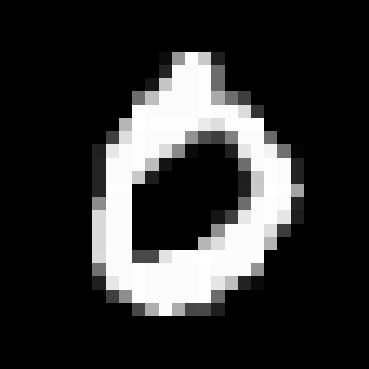
\includegraphics[width=0.18\linewidth]{figures/digits/digits_0.png} & % Adjusted width
    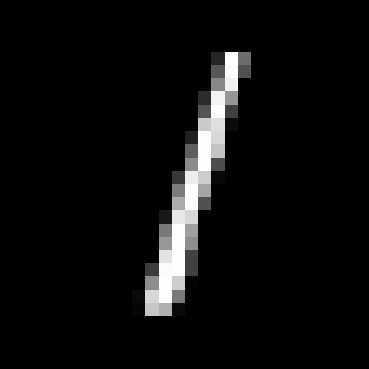
\includegraphics[width=0.18\linewidth]{figures/digits/digits_1.png} & % Adjusted width
    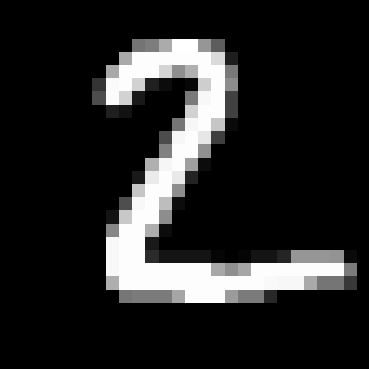
\includegraphics[width=0.18\linewidth]{figures/digits/digits_2.png} & % Adjusted width
    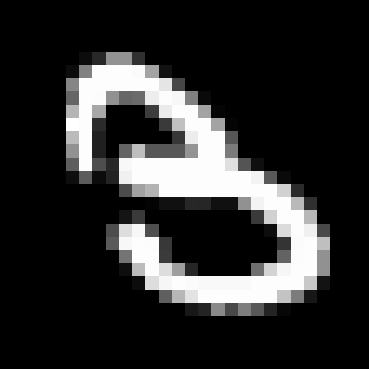
\includegraphics[width=0.18\linewidth]{figures/digits/digits_3.png} & % Adjusted width
    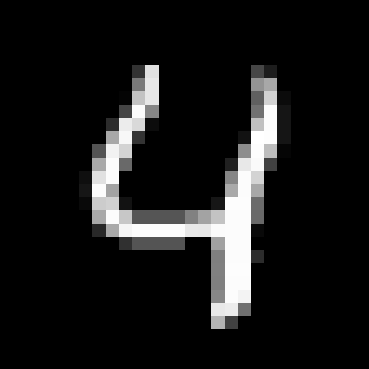
\includegraphics[width=0.18\linewidth]{figures/digits/digits_4.png} \\ % Added newline for next row
    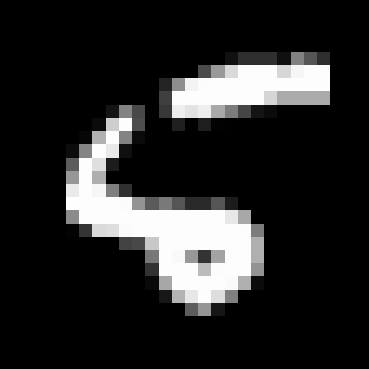
\includegraphics[width=0.18\linewidth]{figures/digits/digits_5.png} & % Adjusted width
    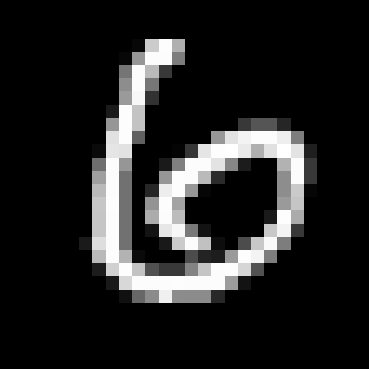
\includegraphics[width=0.18\linewidth]{figures/digits/digits_6.png} & % Adjusted width
    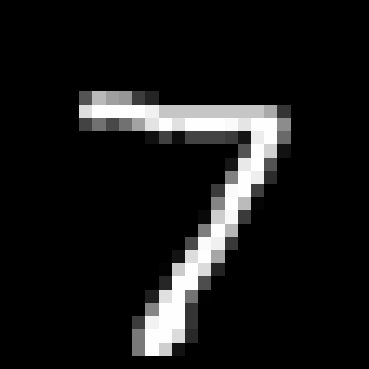
\includegraphics[width=0.18\linewidth]{figures/digits/digits_7.png} & % Adjusted width
    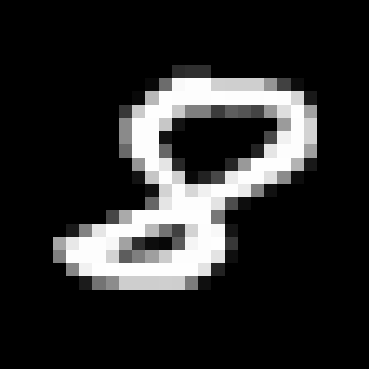
\includegraphics[width=0.18\linewidth]{figures/digits/digits_8.png} & % Adjusted width
    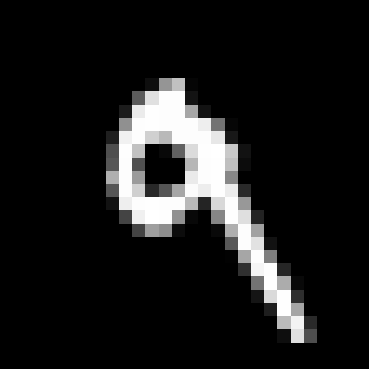
\includegraphics[width=0.18\linewidth]{figures/digits/digits_9.png}   % Adjusted width
  \end{tabular}
  \caption{One representative example per class from the MNIST
           dataset.  Each \(28\times28\) grayscale image is flattened to a
           \(p=784\)-dimensional feature vector before the
           pre-processing pipeline (centering, standardisation, PCA).}
  \label{fig:mnist-examples}
\end{figure}

\paragraph{Pre-processing.}
Real-world data rarely arrive in a form that is optimal for learning.
We apply three light transformations that are standard in pattern
recognition:

\begin{enumerate}[leftmargin=*,label=(\alph*)]
\item \textit{Centring} removes global offsets,
      \(
      \mathbf u_i\!\longmapsto\!
      \mathbf u_i-\bar{\mathbf u},
      \)
      where
      $\bar{\mathbf u}=N^{-1}\sum_{j=1}^{N}\mathbf u_j$.
\item \textit{Standardisation} rescales each feature so that every
      dimension has unit variance, preventing attributes with large
      numerical ranges from dominating the learning process.
\item \textit{Principal-component analysis} (PCA) projects the centred,
      standardised vectors onto the $p'(<p)$ directions of greatest
      variance,
      \(
      \mathbf x_i=\Pi_{\text{PCA}}\mathbf u_i\in\mathbb R^{p'},
      \)
      thereby discarding redundant noise and shrinking the effective
      dimensionality.
\end{enumerate}


\paragraph{Balanced accuracy.}
Performance is summarised through the
\emph{confusion matrix}
$V_{k'k}$, whose entry counts how many test samples belonging to class
$k$ are classified as $k'$.  The
\emph{balanced accuracy} (BA)
\[
\mathrm{BA}=
\frac{1}{K}\sum_{k=1}^{K}\frac{V_{kk}}{N_k}
\]
computes the mean of the per-class accuracies and is robust to class
imbalance. When classes are homogeneous in size, BA reduces to
the usual accuracy.

\paragraph{Classical Nearest-Mean Classifier (CNM-C).}
The nearest-mean classifier (NMC) is a simple, interpretable
classifier that assigns a label to a test sample based on the
\emph{centroid} of the training samples in each class (Fig. \ref{fig:nearest_mean_classifier}).  The
\emph{centroid} of class \(k\) is defined as the mean of the training
samples in that class:

\[
  \boldsymbol\mu_k
  =\frac{1}{N_k}\sum_{i=1}^{N_k}\mathbf u_i,
  \qquad
  \text{where } \mathbf u_i\in C_k.
\]

The CNM classifier assigns a test sample \(\mathbf x\) to the class $j$ if:
\[
    d(\mathbf x,\boldsymbol\mu_j) = \min_{k=1,\dots,K} d(\mathbf x,\boldsymbol\mu_k),
\]

where the distance \(d(\mathbf x, \mathbf y) = \|\mathbf x - \mathbf y\|\) is the Euclidean distance. 
The CNM classifier is simple to implement, as it only requires the computation of the centroids and $K$ distance calculations, one for each centroid.


\begin{figure}[h]
    \centering
    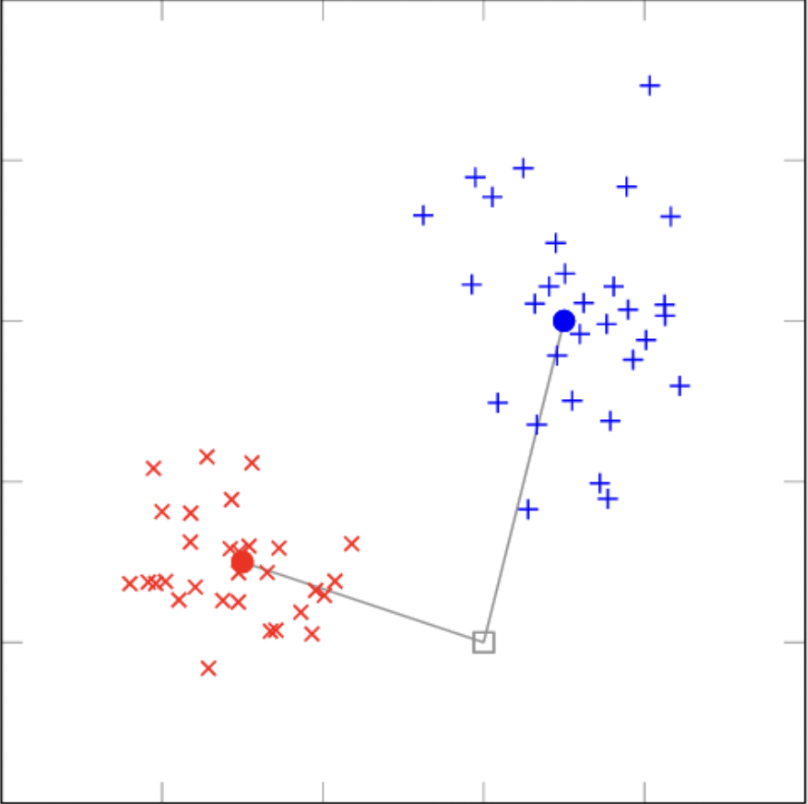
\includegraphics[width=0.6\linewidth]{figures/nearest_mean_classifier.png}
    \caption{Ilustration of the CNM-C decision rule. The training set is split into two classes and the centroids are computed. The nearest centroid to the test sample is selected as the predicted class.}
    \label{fig:nearest_mean_classifier}
\end{figure}

\subsection{Quantum-inspired classification}
\label{subsec:qic}
%--------------------------------------------------------------

Quantum-inspired learning borrows mathematical objects native to
quantum theory—\emph{density operators}, \emph{trace distance},
\emph{superposition}—but applies them on ordinary CPUs/GPUs.  By
embedding classical feature vectors in a Hilbert space, one can exploit
the geometry of quantum states to obtain alternative similarity
measures that sometimes improve accuracy or robustness compared with
purely classical methods~\cite{Sergioli2025}. 
Every quantum-inspired algorithm must start with a function that maps each classical data vector $x$ to a density operator $\rho_x$.  
The choice of this encoding is very important, as it determines the properties of the resulting quantum-inspired algorithm.  

%--------------------------------------------------------------
\paragraph{Density--pattern encodings.}\label{par:encodings}
All quantum-inspired classifiers require a map that
sends a real feature vector \(\mathbf x\in\mathbb R^{d}\) to a
\emph{density operator}
\(\rho_{\mathbf x}= \tilde{\mathbf x}\,
                    \tilde{\mathbf x}^{\!\top}\). There are different ways of doing this mapping:

\begin{enumerate}[leftmargin=*,label=\textbf{(\alph*)}]
%----------------------------------------------------------
\item \textbf{Standard amplitude (SA) encoding.}\\[2pt]
      Normalise the input vector to unit length:
      \[
        \tilde{\mathbf x}^{(\mathrm{SA})}
          =\begin{cases}
             \displaystyle\frac{\mathbf x}{\lVert\mathbf x\rVert},
               &\mathbf x\neq\mathbf 0,\\[6pt]
             (1,0,\dots,0)^{\!\top},&\mathbf x=\mathbf 0.
           \end{cases}
      \]
      The encoded state remains in the original \(d\)-dimensional
      Hilbert space.

%----------------------------------------------------------
\item \textbf{Inverse stereographic (IS) encoding.}\\[2pt]
      Embed \(\mathbf x\) into \(\mathbb R^{d+1}\) through the inverse
      stereographic projection onto the unit sphere:
      \[
        \tilde{\mathbf x}^{(\mathrm{IS})}
           =\frac{1}
                  {1+\lVert\mathbf x\rVert^{2}}
             \Bigl(2x_{1},\dots,2x_{d},
                   \lVert\mathbf x\rVert^{2}-1\Bigr)^{\!\top}.
      \]
      This encoding adds an extra dimension to the input vector, which is
      then projected onto the unit sphere.

%----------------------------------------------------------
\item \textbf{Informative (INF) encoding~\cite{Sergioli2025}.}\\[2pt]
      Attach the norm as an extra amplitude so that both direction and
      length of \(\mathbf x\) affect the representation:
      \[
        \tilde{\mathbf x}^{(\mathrm{INF})}
          =\begin{cases}
             \displaystyle
             \frac{1}{\sqrt{2}}
             \Bigl(\frac{\mathbf x}{\lVert\mathbf x\rVert},\,1\Bigr)^{\!\top},
               &\mathbf x\neq\mathbf 0,\\[8pt]
             (0,\dots,0,1)^{\!\top},
               &\mathbf x=\mathbf 0.
           \end{cases}
      \]
\end{enumerate}

\medskip
For any of the above encodings, the corresponding \emph{density
operator} is obtained by taking the outer product of the encoded
vector with itself:
\[
  \rho_{\mathbf x}= \tilde{\mathbf x}\,
                    \tilde{\mathbf x}^{\!\top}.
\]
This guarantees \(\rho_{\mathbf x}\) is positive semidefinite,
unit-trace, and idempotent (\(\rho_{\mathbf x}^{2}=\rho_{\mathbf x}\)),
hence a valid pure quantum state.
They differ in how much geometric information (direction, norm) is retained, a factor that can
significantly affect classification performance.

\paragraph{Quantum centroid.}
For each class \(k\) with training subset
\(\mathcal S_{k}^{\mathrm{tr}}\), define its \emph{quantum centroid} as the sum of the density operators from the class, divided by the number of elements in the class:

\[
\varrho_{k}=\frac{1}{\lvert\mathcal S_{k}^{\mathrm{tr}}\rvert}
            \sum_{(\mathbf x_i,k)\in\mathcal S_{k}^{\mathrm{tr}}}
            \rho_{\mathbf x_i}.
\]

Unlike the classical centroid, \(\varrho_{k}\) is usually a
\emph{mixed} state and has no direct counterpart in the original
feature space.

\paragraph{Quantum distance measure.}
Similarity between two density patterns is quantified by the
\emph{trace distance},
\[
  d_{\operatorname{tr}}(\rho,\sigma)=
  \tfrac12\operatorname{Tr}\!\bigl|\rho-\sigma\bigr|,
\]
where \(\lvert A\rvert=\sqrt{A^{\dagger}A}\). Note that the trace distance defines a metric; it satisfies the triangle inequality, $d_{tr}(\rho, \sigma) \geq 0$ and $d_{tr}(\rho, \sigma) = d_{tr}(\sigma, \rho)$, and is equal to zero if and only if $\rho = \sigma$.

Having defined the quantum centroid and quantum distance, we can now define the quantum-inspired version of the nearest-mean classifier.

\paragraph{Quantum-inspired nearest-mean classifier (QNM-C).}
The quantum-inspired nearest-mean classifier (QNM-C) is the exact same as the CNM-C, but uses the quantum centroid and quantum distance instead of the classical centroid and Euclidean distance. The algorithm is as follows:
\begin{enumerate}[leftmargin=*,label=(\alph*)]
    \item Encode every training sample \(\mathbf x_i\) as a density operator
      \(\rho_{\mathbf x_i}\) using one of the encodings described in \ref{par:encodings}.

    \item Compute the quantum centroid for each class \(k\):
        \[
            \varrho_{k}=\frac{1}{N_k}\sum_{i=1}^{N_k}\rho_{\mathbf x_i}.
        \]

    \item For each test density operator \(\rho_{\mathbf x}\), assign the class $k$ if 
        \[
            d_{\operatorname{tr}}(\rho_{\mathbf x},\varrho_{k}) = \min_{j=1,\dots,K} d_{\operatorname{tr}}(\rho_{\mathbf x},\varrho_{j}).
        \]
\end{enumerate}

Having defined both the classical and quantum-inspired nearest-mean classifiers, we can now describe the joint transform correlator (JTC) and how it can be used to implement these classifiers optically.

\subsection{Joint Transform Correlator}
\label{subsec:jtc}
A \emph{joint transform correlator} (JTC) is an optical architecture
that performs the cross– and auto–correlation of two 2-D patterns by
means of only \emph{free-space propagation} and \emph{Fourier
transform} lenses, thereby exploiting the inherent parallelism and
picosecond‐scale speed of coherent light.  Unlike classical
Vander~Lugt correlators, the JTC dispenses with a pre-fabricated
matched filter: both the \emph{reference} pattern \(s_{1}(x,y)\) and
the \emph{query} pattern \(s_{2}(x,y)\) are displayed side-by-side in
the same input plane~\cite{Javidi1989}.

\paragraph{Operational principle.}
Let the two patterns be centred at \(\pm x_{0}\) along the horizontal
axis, i.e.\ \(s_{1}(x+x_{0},y)\) and \(s_{2}(x-x_{0},y)\).  A
\(1f\)-configuration lens (focal length \(f\)) produces at its back
focal plane the joint Fourier transform
\[
  G(\alpha,\beta)=
    S_{1}\!\bigl(\tfrac{\alpha}{\lambda f},
                 \tfrac{\beta}{\lambda f}\bigr)\,
      e^{-i2\pi x_{0}\alpha/\lambda f}
  + S_{2}\!\bigl(\tfrac{\alpha}{\lambda f},
                 \tfrac{\beta}{\lambda f}\bigr)\,
      e^{+i2\pi x_{0}\alpha/\lambda f},
\]
where \((\alpha,\beta)\) are spatial-frequency coordinates and
\(S_{j}\) denotes the Fourier transform of \(s_{j}\).
A photosensor records the \emph{joint power spectrum}
\(|G|^{2}\); its intensity contains four beating terms:

\[
  |G|^{2}
  =|S_{1}|^{2}+|S_{2}|^{2}
   +S_{1}S_{2}^{\!*}e^{-i4\pi x_{0}\alpha/\lambda f}
   +S_{2}S_{1}^{\!*}e^{+i4\pi x_{0}\alpha/\lambda f}.
\]

A second lens takes the inverse Fourier transform of this intensity
pattern.  The constant terms yield \emph{autocorrelation}
peaks near the optic axis, whereas the two cross-terms produce a pair
of off-axis peaks located at \((\pm2x_{0},0)\) whose heights are
proportional to the cross-correlation
\(s_{1}\star s_{2}\).  Detecting the peak energy therefore reveals the
similarity between the two input patterns.

TODO: INCLUDE A DIAGRAM OF THE JTC, AND THE CORRELATION PLANE, AS WELL AS SOME EXAMPLES OF CORRELATION (SHIFTED IMAGE VS ORIGINAL, ROTATED VS ORIGINAL, AND CORRELATION VALUES)

%------------------------------------------------------
\begin{figure}[htbp]
  \centering
  \begin{subfigure}[b]{\linewidth}
    \centering
    \includegraphics[width=\linewidth]%
      {figures/correlation/original_vs_shifted_corr_plane.png}
    \caption{Original image vs.\ shifted copy}%
    \label{fig:corr-shifted}
  \end{subfigure}
  \hfill
  \begin{subfigure}[b]{\linewidth}
    \centering
    \includegraphics[width=\linewidth]%
      {figures/correlation/original_vs_random_corr_plane.png}
    \caption{Original image vs.\ random image}%
    \label{fig:corr-random}
  \end{subfigure}

  \caption{Correlation-plane intensity produced by the joint transform
           correlator: (a) shows two strong off-axis peaks because the
           query is a shifted version of the reference, whereas (b)
           shows no significant peaks for an unrelated image.}%
  \label{fig:jtc-diagram}
\end{figure}
%------------------------------------------------------

\subsection{Optical implementations of the classifiers}
\label{subsec:optical-qnm}

The


\section{Results}

\begin{table}[htbp]
  \centering
  \caption{Classification accuracy (mean $\pm$ std.)}
  \label{tab:cls-results}
  \begin{tabular}{@{}lll c@{}}
    \toprule
    Classifier & Distance metric & Encoding & Accuracy (\%)\\ 
    \midrule
    RBF-C & Euclidean & - & - \\
    RBF-C & JTC & - & - \\[2pt]
    CNM-C & Euclidean & — & $80.38 \pm 0.38$ \\ 
    CNM-C & JTC & — & $72.42 \pm 0.55$ \\[2pt]
    QNM-C & Trace     & Standard     & \textbf{$85.84 \pm 0.38$} \\ 
    QNM-C & Fidelity  & Standard     & $78.77 \pm 0.34$ \\[2pt]
    QNM-C & Trace     & Informative  & $81.26 \pm 0.37$ \\ 
    QNM-C & Fidelity  & Informative  & \textbf{$82.39 \pm 0.40$} \\ 
    \bottomrule
  \end{tabular}
\end{table}




\section{Data Encoding}
\subsection{Gram Matrix Encoding}

We consider a column vector $u$ representing an image sample. To embed this into a higher-order representation, we construct the normalized outer product:
\[
\rho = \frac{uu^T}{\text{Tr}(uu^T)}
\]
This yields a density-like matrix $\rho$ with trace 1, encoding pairwise correlations between pixels. Such an encoding is inspired by quantum mechanical density operators and preserves structural information in the image.

\begin{figure}[h!]
    \centering
    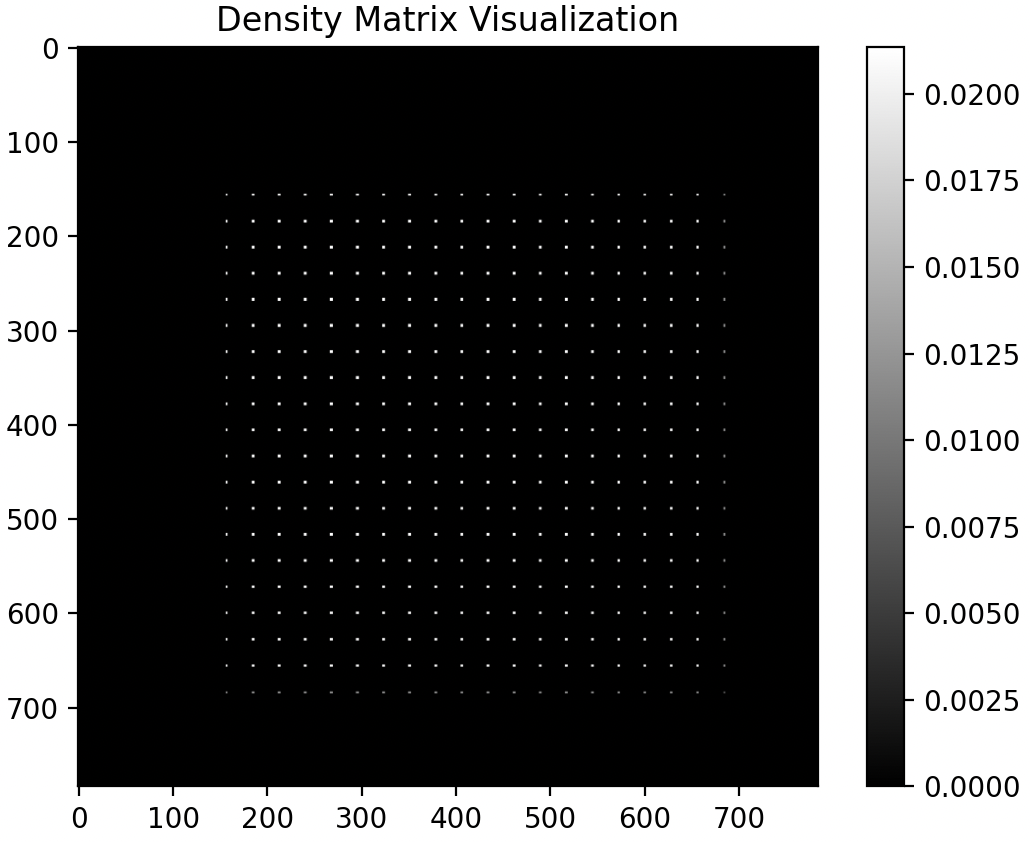
\includegraphics[width=0.6\linewidth]{figures/density_matrix_nmist_one.png}
    \caption{Gram matrix encoding $\rho$ of the digit 1 image}
    \label{fig:density_matrix}
\end{figure}

\section{Radial Basis Function Network}

RBF networks model the hypothesis function $h(x)$ using a radial function centered around key points (called \emph{centers}). Each center influences the prediction based on its proximity to the input $x$. The standard form is:
\[
h(x) = \sum_{n=1}^N w_n\exp\left(-\gamma\| x - x_n \|^2\right)
\]
where $\gamma$ determines the width of the radial functions, and $w_n$ are the learned weights.

\subsection{Exact Interpolation}
Given training data $D = \{(x_1, y_1), \dots, (x_N, y_N)\}$, we can formulate the interpolation condition:
\[
\sum_{m=1}^N w_m\exp\left(-\gamma\| x_n - x_m \|^2\right) = y_n, \quad \forall n
\]
In matrix notation:
\[
\Phi \mathbf{w} = \mathbf{y}, \quad \text{where } \Phi_{n,m} = \exp\left(-\gamma\|x_n - x_m\|^2\right)
\]
If $\Phi$ is invertible, we can directly solve:
\[
\mathbf{w} = \Phi^{-1} \mathbf{y}
\]
This yields an exact interpolating function.

\subsection{Classification}
For classification, we apply a decision rule such as:
\[
h(x) = \operatorname{sign}\left(\sum_{n=1}^N w_n\exp(-\gamma\|x - x_n\|^2)\right)
\]
In multi-class settings, this can be extended to a softmax output over class scores.

\subsection{Training with Least Squares}
Instead of enforcing exact interpolation, we may use a least squares approach to minimize:
\[
E = \sum_{n=1}^N (h(x_n) - y_n)^2
\]
This leads to the ridge-regularized solution:
\[
\mathbf{w} = (\Phi^T\Phi + \lambda I)^{-1}\Phi^T \mathbf{y}
\]
where $\lambda$ is a regularization parameter.

\section{Choosing RBF Centers}
Using every data point as a center is computationally expensive. Instead, we reduce the number of centers to $K \ll N$ by clustering the dataset using \textbf{K-Means}:

We define:
\[
J = \sum_{k=1}^K \sum_{x_n \in S_k} \| x_n - \mu_k \|^2
\]
and use Lloyd's algorithm to iteratively minimize $J$:
\begin{align*}
\mu_k &= \frac{1}{|S_k|}\sum_{x_n \in S_k} x_n \\
S_k &= \{ x_n : \|x_n - \mu_k\| \leq \|x_n - \mu_j\|,\ \forall j \neq k \}
\end{align*}

Repeat these steps until convergence. Since the process is sensitive to initialization, we typically run K-Means multiple times and choose the best clustering.

\begin{figure}[h!]
    \centering
    % Consider plotting a 3D Gaussian RBF here with Gnuplot
    \begin{gnuplot}[scale=0.6, terminal=pdf]
set title "3D Gaussian Function"
set xlabel "x"
set ylabel "y"
set zlabel "z"
set hidden3d
set view 60, 80
set isosamples 50, 50
set xrange [-5:5]
set yrange [-5:5]

# Parameters for the Gaussian
sigma = 1.0
mu_x = 0.0
mu_y = 0.0

# 2D Gaussian Function
gaussian(x, y) = exp(-((x - mu_x)**2 + (y - mu_y)**2) / (2 * sigma**2))

splot gaussian(x, y) with lines palette
\end{gnuplot}
    \caption{Example of a Gaussian RBF centered at $\mu$}
    \label{fig:gaussian_rbf}
\end{figure} 

\section{Implementation Notes}
The RBF network was implemented in Python using NumPy and scikit-learn. To avoid memory issues, we:
\begin{itemize}
    \item Use MiniBatchKMeans to find centers efficiently.
    \item Use perceptron-based or regularized least squares learning.
    \item Avoid computing large $\Phi^T\Phi$ matrices when possible.
\end{itemize}

\section{Optical Im}

\section{Conclusion}
RBF networks provide an elegant and powerful framework for classification. Through Gaussian kernel construction and data-driven center selection, they can adapt to local structures in the data. When combined with efficient encodings such as Gram matrices and practical training algorithms, they scale to real-world tasks like digit recognition.

\bibliography{references}{}
\bibliographystyle{plain}

\end{document}
